\subsection{Thuật toán so khớp LightGlue}

Thuật toán LightGlue \cite{lindenberger2023LightGlue} là một mạng nơ-ron sâu được thiết kế để thực hiện việc khớp các đặc trưng cục bộ giữa các cặp ảnh, với mục tiêu cải thiện hiệu quả và độ chính xác so với các phương pháp truyền thống. LightGlue được phát triển dựa trên nền tảng của SuperGlue \cite{sarlin2020superglue} – một mô hình tiên tiến trong lĩnh vực so khớp đặc trưng – LightGlue mang đến những cải tiến đáng kể về hiệu suất tính toán, độ chính xác, và khả năng huấn luyện. Đặc biệt, LightGlue có khả năng thích ứng với độ khó của bài toán, giúp giảm thời gian suy luận trên các cặp ảnh dễ khớp. LightGlue đang được ưa chuộng sử dụng cho nhiều các bài toán thực tế như định vị robot, xây dựng bản đồ, tái tạo 3D,...

\textbf{Bản chất ý tưởng và mô hình}

LightGlue được xây dựng dựa trên kiến trúc Transformer, tận dụng cơ chế tự chú ý và chú ý chéo để tăng cường khả năng khớp đặc trưng. Ý tưởng cốt lõi của LightGlue là tối ưu hóa quá trình khớp đặc trưng bằng cách giảm thiểu các phép tính không cần thiết thông qua hai cơ chế chính:

\begin{itemize}
    \item Dừng sớm: LightGlue sử dụng một bộ phân loại độ tin cậy để đánh giá mức độ tin cậy của các dự đoán tại mỗi tầng của mạng. Nếu dự đoán tại một tầng sớm đạt độ tin cậy cao, quá trình suy luận sẽ dừng lại, giúp tiết kiệm thời gian tính toán.
    \item Cắt tỉa điểm đặc trưng: Các điểm đặc trưng được dự đoán là không thể khớp sẽ bị loại bỏ sớm khỏi quá trình suy luận, giảm số lượng phép tính trong các tầng sau.
\end{itemize}

\begin{figure}[H]
    \centering
    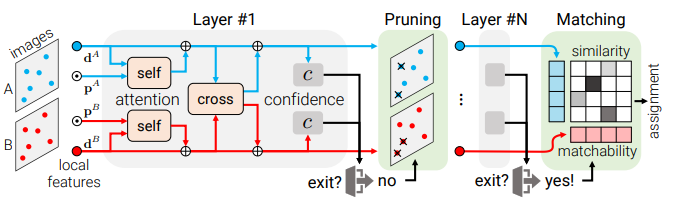
\includegraphics[width=\linewidth]{figures/c3/kien_truc_light_glue.png}
    \caption{Kiến trúc mạng thuật toán so khớp LightGlue \cite[Fig.~3]{lindenberger2023LightGlue}.}
    \label{fig:lightglue}
\end{figure}

Mô hình LightGlue nhận đầu vào là tập hợp các điểm đặc trưng và véc-tơ mô tả đặc trưng tương ứng. Quá trình so khớp được minh họa ở Hình \ref{fig:lightglue} bao gồm các bước sau:

\begin{itemize}
    \item Khởi tạo đặc trưng ban đầu: Các điểm đặc trưng từ hai ảnh được biểu diễn dưới dạng tập hợp $\mathcal{F}_0 = \{(\mathbf{k}_i^0, \mathbf{d}_i^0)\}_{i=1}^{N_0}$ và $\mathcal{F}_1 = \{(\mathbf{k}_j^1, \mathbf{d}_j^1)\}_{j=1}^{N_1}$, trong đó $\mathbf{k}_i^0, \mathbf{k}_j^1 \in \mathbb{R}^2$ là tọa độ điểm đặc trưng, và $\mathbf{d}_i^0, \mathbf{d}_j^1 \in \mathbb{R}^D$ là các vector mô tả đặc trưng. Tại bước này, các vector mô tả đặc trưng được mã hóa thêm thông tin vị trí để tăng cường khả năng biểu diễn không gian:
    \begin{equation}
        \mathbf{x}_i^0 = \mathbf{d}_i^0 + \text{PE}(\mathbf{k}_i^0), \quad \mathbf{x}_j^1 = \mathbf{d}_j^1 + \text{PE}(\mathbf{k}_j^1),
    \end{equation}
    trong đó $\text{PE}(\cdot)$ là hàm mã hóa vị trí.

    \item Tăng cường ngữ cảnh qua tự chú ý: 
    Mỗi tập đặc trưng $\mathcal{F}_0$ và $\mathcal{F}_1$ được xử lý độc lập thông qua các tầng tự chú ý trong Transformer để tích hợp thông tin ngữ cảnh cục bộ từ các điểm đặc trưng lân cận trong cùng một ảnh. Quá trình này được biểu diễn như sau:
    \begin{equation}
        \mathbf{x}_i^{0'} = \text{SelfAttention}(\mathbf{x}_i^0, \{\mathbf{x}_k^0\}_{k=1}^{N_0}; \theta_s),
    \end{equation}
    trong đó $\theta_s$ là tham số của mô-đun tự chú ý. Tương tự cho $\mathcal{F}_1$. Bước này giúp các đặc trưng trở nên phong phú hơn bằng cách học mối quan hệ giữa các điểm trong cùng một ảnh.

    \item Tích hợp thông tin qua chú ý chéo: 
    Sau khi tăng cường ngữ cảnh cục bộ, LightGlue sử dụng cơ chế chú ý chéo để trao đổi thông tin giữa hai ảnh. Điều này cho phép mỗi điểm đặc trưng ở một ảnh tham khảo các đặc trưng tiềm năng ở ảnh kia:
    \begin{equation}
        \mathbf{x}_i^{0''} = \text{CrossAttention}(\mathbf{x}_i^{0'}, \{\mathbf{x}_j^{1'}\}_{j=1}^{N_1}; \theta_c),
    \end{equation}
    trong đó $\theta_c$ là tham số của mô-đun chú ý chéo. Bước này rất quan trọng để xác định các cặp điểm đặc trưng tiềm năng giữa hai ảnh.

    \item Cập nhật đặc trưng qua các tầng: 
    LightGlue áp dụng nhiều tầng Transformer (thường từ 6 đến 9 tầng), mỗi tầng bao gồm cả tự chú ý và chú ý chéo, để tinh chỉnh các đặc trưng. Sau mỗi tầng, một bộ phân loại độ tin cậy đánh giá xác suất khớp của các điểm đặc trưng:
    \begin{equation}
        p_i = \sigma(\text{MLP}(\mathbf{x}_i^{0''}; \theta_p)),
    \end{equation}
    trong đó $\sigma$ là hàm sigmoid, và $\theta_p$ là tham số của mạng MLP. Các điểm có xác suất thấp sẽ bị loại bỏ (cắt tỉa), và nếu toàn bộ dự đoán đạt ngưỡng tin cậy, quá trình suy luận có thể dừng sớm.

    \item Dự đoán ma trận khớp: 
    Sau khi xử lý qua các tầng, LightGlue xây dựng ma trận điểm số khớp $\mathbf{S} \in \mathbb{R}^{N_0 \times N_1}$, trong đó:
    \begin{equation}
        \mathbf{S}_{ij} = \langle \mathbf{x}_i^{0''}, \mathbf{x}_j^{1''} \rangle,
    \end{equation}
    với $\langle \cdot, \cdot \rangle$ là tích vô hướng hoặc một hàm đo tương tự được học. Ma trận $\mathbf{S}$ được chuẩn hóa thành ma trận xác suất khớp $\mathbf{P}$ bằng cách sử dụng thuật toán Sinkhorn hoặc phương pháp tối ưu hóa khác \cite{lindenberger2023LightGlue}:
    \begin{equation}
        \mathbf{P} = \text{Sinkhorn}(\mathbf{S}; \tau),
    \end{equation}
    trong đó $\tau$ là tham số điều chỉnh độ mượt của phân phối xác suất. Ma trận $\mathbf{P}$ sau đó được sử dụng để xác định các cặp điểm đặc trưng tương ứng thông qua giá trị ngưỡng (thường là 0.5) hoặc lấy tối đa.

    % Thuật toán Sinkhorn lặp lại quá trình chuẩn hóa hàng và cột để đảm bảo $\mathbf{P}$ là ma trận doubly stochastic (tổng các hàng và cột bằng 1):
    % \begin{equation}
    %     \mathbf{P}^{(t+1)} = \text{Norm}_{\text{row}}\left( \exp(\mathbf{S}/\tau) \cdot \text{Norm}_{\text{col}}(\mathbf{P}^{(t)}) \right),
    % \end{equation}
    % trong đó $\text{Norm}_{\text{row}}$ và $\text{Norm}_{\text{col}}$ là các phép chuẩn hóa theo hàng và cột, $\tau$ là tham số điều chỉnh độ mượt, và $t$ là số lần lặp. Sau một số lần lặp, $\mathbf{P}$ hội tụ đến một ma trận xác suất khớp.
    
    \item Tinh chỉnh và xuất kết quả: 
    Các cặp điểm khớp được tinh chỉnh bằng cách kiểm tra độ nhất quán hình học hoặc áp dụng các bộ lọc bổ sung (ví dụ, RANSAC) để loại bỏ các khớp sai. Kết quả cuối cùng là tập hợp các cặp điểm đặc trưng tương ứng giữa hai ảnh.
\end{itemize}

\textbf{Điểm mạnh}

LightGlue sở hữu nhiều ưu điểm nổi bật:

\begin{itemize}
    \item Hiệu quả tính toán: Nhờ cơ chế dừng sớm và cắt tỉa điểm, LightGlue giảm đáng kể thời gian suy luận, đặc biệt trên các cặp ảnh có độ chồng lấn lớn hoặc ít thay đổi về ngoại quan. Thử nghiệm cho thấy LightGlue đạt tốc độ 20 FPS với 512 điểm đặc trưng trên CPU Intel i7 10700K \cite{lindenberger2023LightGlue}.
    \item Độ chính xác cao: LightGlue vượt trội so với các phương pháp khác trong các bài kiểm tra chuẩn như IMC 2021 Phototourism, với AUC trung bình 58/70 cho tác vụ đa góc nhìn khi kết hợp với DISK \cite{lindenberger2023LightGlue}.
    \item Tính thích ứng: LightGlue tự động điều chỉnh độ sâu (số tầng) và độ rộng (số điểm đặc trưng) dựa trên độ khó của cặp ảnh, tối ưu hóa hiệu suất trong các kịch bản thực tế.
\end{itemize}

\textbf{Điểm yếu}

Mặc dù có nhiều ưu điểm, LightGlue vẫn tồn tại một số hạn chế:

\begin{itemize}
    \item Phụ thuộc vào chất lượng đặc trưng đầu vào: Hiệu suất của LightGlue phụ thuộc lớn vào chất lượng của các điểm đặc trưng và mô tả tử được trích xuất bởi các thuật toán như SuperPoint hoặc DISK. Trong điều kiện ánh sáng yếu hoặc ảnh có nhiễu cao, hiệu quả của LightGlue có thể bị giảm \citep{Li2024Improved}.
    \item Hiệu suất bị hạn chế khi số lượng điểm đặc trưng lớn.
\end{itemize}

LightGlue là một bước tiến quan trọng trong lĩnh vực khớp đặc trưng cục bộ, mang lại sự cân bằng tối ưu giữa hiệu quả tính toán và độ chính xác. Với kiến trúc Transformer linh hoạt và các cơ chế thích ứng thông minh, LightGlue mở ra tiềm năng lớn cho các ứng dụng thời gian thực như tái tạo 3D, định vị và lập bản đồ. Trong luận văn này, tôi sẽ thực nghiệm sử dụng LightGlue kết hợp với thuật toán trích xuất đặc trưng ALIKED nhằm cải tiến độ chính xác cho quy trình SfM truyền thống với SIFT cho đối tượng cột ăng-ten.